The parameter for this distribution was $\beta=-2.75$ with a distribution looking like this

\begin{figure}[h]
      \caption{Distribution of a random powerlaw input with $\beta=-2.75$}
      \centering
      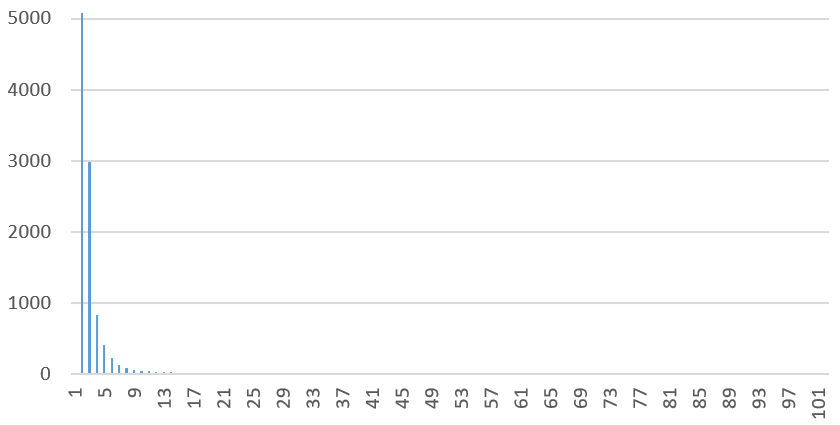
\includegraphics[width=0.7\textwidth]{figures/images/numberGenerator/powerlaw_-2_75.png}\label{fig:powerDistExample1}
\end{figure}

For a value of $\beta=-1.25$ the distribution looks a bit different.
There are less small values close to one and instead also big values even over 1000.
Figure~\ref{fig:powerDistExample2} is cropped to get a more clear view for the smaller values.
The higher values mostly occurred 0 to 2 times.
The highest value 8848 occurred only once.

\begin{figure}[h]
      \caption{Distribution of a random powerlaw input with $\beta=-1.25$}
      \centering
      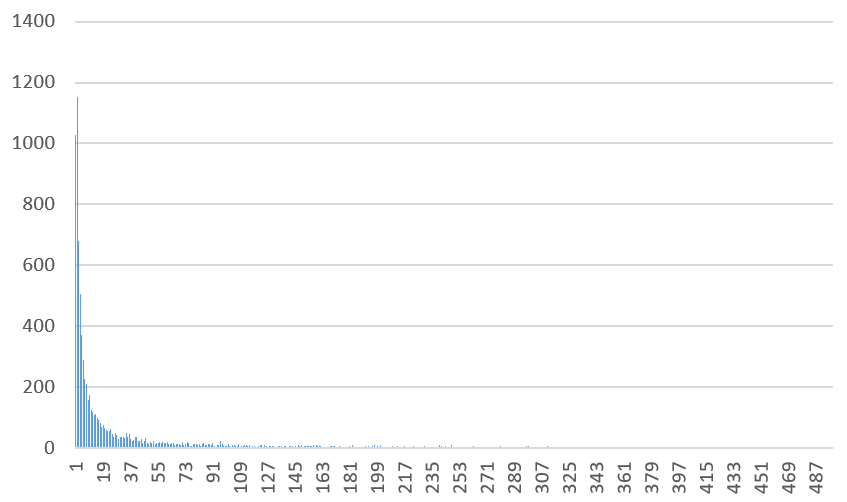
\includegraphics[width=0.7\textwidth]{figures/images/numberGenerator/powerlaw_-1_25.png}\label{fig:powerDistExample2}
\end{figure}